\section{Training Pipeline}

UrbanDreamer follows a two-stage training pipeline.  The first stage provides warmup learning for the dynamics model. The second stage
alternates real simulator collection, causal HDV-response learning, online
world-model updates, and imagined actor-critic optimization after every
collected episode. Consequently, the model is continually adapted to the
state-action distribution induced by the improving CAV policy, while policy
learning remains grounded in newly observed traffic transitions.
% 中文注释：UrbanDreamer 采用两阶段训练流程。第一阶段为 traffic world model 提供稳定的初始化。第二阶段在每个 collected episode 之后，依次交替进行 real simulator collection、causal HDV-response learning、online world-model updates 和 imagined actor-critic optimization。因此，world model 会持续适应不断改进的 CAV policy 所诱导的 state-action distribution，而 policy learning 仍以新观测到的 traffic transitions 为基础。

\subsubsection{Offline Warmup}

Before online policy learning, we collect a fixed set of transitions from the simulator using exploratory CAV route choices. The encoder, flow-matching dynamics, and decoder are
then fitted on these transitions using \(\mathcal{L}_\phi\). 
% 中文注释：在 online policy learning 之前，我们从 post-mutation simulator state 收集一组固定 transitions；该阶段使用 exploratory CAV route choices，并冻结 HDV adaptation。随后，encoder、flow-matching dynamics 和 decoder 使用 \(\mathcal{L}_\phi\) 在这些 transitions 上完成初始化训练。causal HDV response predictor 不在该阶段训练，因为固定 collection 不能表示由持续变化的 CAV policy 引起的 episode-to-episode response。actor、critics 和 response predictor 在逐 episode online stage 开始时初始化。

\subsubsection{Online Training}

During online collection, HDV adaptation is enabled and the current actor
stochastically samples a valid route for every active CAV.  The same sampled
one-hot decision is used to reroute the vehicle, construct
\(\Psi_{e,t}^{\mathrm{CAV}}\), and store the world-model action in replay.
This action alignment ensures that each observed transition is paired with the
physical CAV intervention that actually produced it.  Deterministic masked
argmax is reserved for simulator evaluation rather than training collection.
% 中文注释：在 online collection 中，HDV adaptation 被启用，current actor 为每辆 active CAV 随机采样一条有效 route。同一个 sampled one-hot decision 同时用于对车辆执行 rerouting、构造 \(\Psi_{e,t}^{\mathrm{CAV}}\)，以及在 replay 中保存 world-model action。这样的 action alignment 保证每个 observed transition 都与实际产生它的物理 CAV intervention 配对。deterministic masked argmax 仅用于 simulator evaluation，而不用于 training collection。

Only episodes satisfying the replay acceptance criterion are admitted to the
bounded world-model replay buffer \(\mathcal{B}\).  Before the observed target
\(H_e^\star\) of an accepted episode is exposed to the response predictor,
\(\hat H_e^{\mathrm{HDV}}\) is computed using only summaries from preceding
episodes and is attached to that episode's transitions.  After
\(H_e^\star\) is recorded, the predictor is updated on the available adjacent
episode pairs using \(\mathcal{L}_\psi\), and the world model is independently
updated on real transition minibatches from \(\mathcal{B}\) using
\(\mathcal{L}_\phi\).  This ordering prevents the current HDV target from
leaking into its own causal prediction.
% 中文注释：只有满足 replay acceptance criterion 的 episodes 才会进入有界的 world-model replay buffer \(\mathcal{B}\)。在 accepted episode 的 observed target \(H_e^\star\) 暴露给 response predictor 之前，\(\hat H_e^{\mathrm{HDV}}\) 只根据先前 episodes 的 summaries 计算，并附加到当前 episode 的 transitions 上。记录 \(H_e^\star\) 后，predictor 使用 \(\mathcal{L}_\psi\) 在已有的 adjacent episode pairs 上更新；world model 则使用 \(\mathcal{L}_\phi\) 在从 \(\mathcal{B}\) 采样的 real transition minibatches 上独立更新。这个顺序防止 current HDV target 泄漏到它自身的 causal prediction 中。

The main online configuration does not apply a direct actor update to real
simulator returns.  Instead, valid CAV decision states are sampled from
\(\mathcal{B}\) to initialize the vehicle-level imagined rollouts described
above.  Within each rollout, the actor samples masked route actions, the same
one-hot actions define the vehicle wrapper and graph-level CAV pressure, and
the world model predicts the resulting traffic evolution.  The resulting
per-vehicle and global lambda returns jointly update the actor and both
critics.
% 中文注释：当前 online 主线不直接使用 real simulator returns 更新 actor。相反，训练从 \(\mathcal{B}\) 中采样包含有效 CAV decisions 的 states，并用它们初始化前文介绍的 vehicle-level imagined rollouts。在每个 rollout 内，actor 采样 masked route actions；相同的 one-hot actions 同时用于 vehicle wrapper 和 graph-level CAV pressure；world model 则预测由这些 actions 导致的 traffic evolution。最终得到的 per-vehicle 和 global lambda returns 共同用于更新 actor 和两个 critics。

\begin{algorithm}[t]
\caption{Online training}
\label{alg:urbandreamer}
\small
\begin{algorithmic}
\REQUIRE Road graph \(G\), simulator, training-episode budget, checkpoint indices
\ENSURE Simulator-selected CAV route actor \(\pi_\theta\)
\FOR{each online episode \(e\)}
  \STATE Collect one simulator episode using masked stochastic route samples from \(\pi_\theta\)
  \STATE Reuse each sampled one-hot route for execution, \(\Psi_{e,t}^{\mathrm{CAV}}\), and replay
  \IF{the episode satisfies the replay acceptance criterion}
    \STATE Predict \(\hat H_e^{\mathrm{HDV}}\) from preceding episode summaries
    \STATE Attach \(\hat H_e^{\mathrm{HDV}}\), append the episode to \(\mathcal{B}\), and discard stale transitions
    \STATE Update \(g_\psi^{\mathrm{HDV}}\) on available adjacent episode pairs
  \ENDIF
  \IF{a world-model update is scheduled and \(\mathcal{B}\) is nonempty}
    \FOR{each configured world-model update}
      \STATE Sample real transitions from \(\mathcal{B}\) and minimize \(\mathcal{L}_\phi\)
    \ENDFOR
  \ENDIF
  \IF{\(\mathcal{B}\) contains enough valid CAV decision states}
    \FOR{each configured imagined actor-critic update}
      \STATE Sample replay start states and initialize their vehicle states
      \FOR{each of the next \(L_{\mathrm{im}}\) imagined decisions}
        \STATE Sample masked routes from \(\pi_\theta\) and construct \(\Psi_t^{\mathrm{CAV}}\)
        \STATE Predict \(Z_{t+1}\) using the stored causal HDV context
        \STATE Advance the vehicle wrapper and record rewards and active masks
      \ENDFOR
      \STATE Compute lambda returns and update the actor and both critics
    \ENDFOR
  \ENDIF
  \IF{\(e\) is a checkpoint episode}
    \STATE Save the actor, critics, world model, and response predictor
  \ENDIF
\ENDFOR
\STATE Evaluate saved actors in the simulator using masked argmax routes
\RETURN The actor with the lowest global mean travel time
\end{algorithmic}
\end{algorithm}
% 中文注释：Algorithm~\ref{alg:urbandreamer} 首先在冻结 HDV adaptation 的固定 warm-up transitions 上初始化 world model。进入 online stage 后，每个 episode 都使用 current actor 的 masked stochastic route samples 进行 simulator collection，并将同一个 sampled one-hot route 用于车辆执行、planned CAV pressure 和 replay。满足 acceptance criterion 的 episode 会先得到仅依赖先前 episode summaries 的 causal HDV prediction，再进入 bounded replay；随后分别更新 HDV response predictor 和 world model。当 replay 中存在足够的有效 CAV decision states 时，算法从 replay 初始化 imagined rollouts，在每一步采样 route、推进 world model 和 vehicle wrapper，并根据 lambda returns 联合更新 actor 与两个 critics。训练完成后，所有 saved actors 使用 masked argmax 在 simulator 中评估，并按照 global mean travel time 选择最终 actor。

At designated episodes, UrbanDreamer saves the actor, critics, world model,
and response predictor together.  After online training, each saved actor is
evaluated in the real simulator with masked argmax route selection, and the
checkpoint with the lowest global mean travel time is selected.  Simulator
selection prevents favorable world-model errors from determining the final
policy solely through imagined returns.
% 中文注释：在指定 episodes，UrbanDreamer 会同时保存 actor、critics、world model 和 response predictor。online training 完成后，每个 saved actor 都使用 masked argmax route selection 在真实 simulator 中评估，并选择 global mean travel time 最低的 checkpoint。基于 simulator 的选择可以防止有利于 policy 的 world-model errors 仅通过 imagined returns 决定最终 policy。


\section{Experimental Settings}
\label{app:exp-settings}

\paragraph{Benchmarks.}  Table~\ref{tab:benchmarks} summarizes the three urban
networks.  All methods use the same departure demand, candidate route
generator (\(K=4\) candidates per decision), and incident configuration.  The
incident speed caps are applied to all lanes of the selected edges during the
indicated window and are removed afterwards; the decision interval is 60~s
for all networks.

\begin{table}[h]
  \centering
  \caption{Benchmark statistics.}
  \renewcommand{\arraystretch}{1.0}
  \resizebox{\columnwidth}{!}{
    \begin{tabular}{lccc}
      \toprule
      & Gretz-Armainvilliers & Ingolstadt & Fontenay-en-Parisis \\
      \midrule
      Road segments & 4,485 & 853 & 7,585 \\
      Scheduled vehicles & 636 & 1,035 & 2,068 \\
      CAVs / HDVs & 254 / 382 & 414 / 621 & 827 / 1,241 \\
      Incident edges & 1 & 1 & 7 \\
      Incident window (s) & [500, 2500) & [500, 1500) & [300, 1800) \\
      Speed cap (m/s) & 0.1 & 1.0 & 0.1 \\
      \bottomrule
    \end{tabular}
  }
  \label{tab:benchmarks}
\end{table}

\paragraph{Training and evaluation protocol.}  The world-model warm-up
collects 50 exploratory episodes in which every CAV follows an
\(\epsilon\)-greedy routing rule (\(\epsilon=0.4\)).  All methods are trained
for 500 episodes per network under the same protocol, saving checkpoints
every 25 episodes.  Each checkpoint is then evaluated with
the same masked stochastic route sampling used in collection, running enough
held-out episodes for the HDV day-to-day route-choice probabilities to
stabilize, and the reported results correspond to the final checkpoint after
convergence.  All runs use a single NVIDIA RTX 3090 GPU.

\paragraph{Toy network.}  The scalability profile additionally includes a
small synthetic Toy network with 24 registered road segments and the same
decision interval and CAV penetration as the real networks.  It serves only
as the smallest pilot point in
Figure~\ref{fig:scalability_training_time} and is not used in any other
experiment.

\section{Baseline Implementations}
\label{app:baselines}

All learning baselines use the same route-candidate observations and valid
candidate masks as UrbanDreamer, and are trained on the same episodes under
the protocol of Appendix~\ref{app:exp-settings}.

\paragraph{Greedy heuristics.}  Free-flow greedy and live-current greedy are
training-free: at each decision they select the valid candidate with the
smallest sum of free-flow or current segment travel times, respectively.

\paragraph{IQL.}  Independent Q-learning with a parameter-shared Q-network
over the route observations.  Exploration is \(\epsilon\)-greedy over valid
candidates, with \(\epsilon\) decayed from \(0.99\) to \(0.05\) per decision.

\paragraph{IPPO.}  Independent PPO with a parameter-shared actor--critic,
probability-ratio clip \(0.2\), and entropy regularization; each CAV learns
from its own transitions.

\paragraph{MAPPO.}  The same decentralized actor as IPPO, trained with a
centralized critic that reads the joint traffic state and outputs a value for
each vehicle slot (three hidden layers of width 64).

\paragraph{MAMBA.}  A Dreamer-style multi-agent model-based baseline using
the upstream architecture defaults: a per-agent discrete latent state model
(\(32\times32\) categoricals) with transformer dynamics (3 layers, 8 heads),
imagination horizon 15, and PPO clip \(0.075\).  Its world model is first
warmed up on 41 exploratory episodes before online training.  Unlike
UrbanDreamer, MAMBA's
learned model is agent-centric: it does not model the segment-level traffic
field or the HDV demand, and its world model, actor, and critic are trained
from the same online episodes as the other baselines.

\section{HDV Adaptation in the Simulator}
\label{app:hdv-adaptation}

Each HDV belongs to one origin--destination (OD) pair with \(K=4\) candidate
routes generated by the same route generator used for CAVs.  At its departure
time, an HDV samples one route from the current per-OD route-choice
probabilities and keeps it for the rest of the episode.  After each episode,
the probabilities of every OD pair are updated once in the day-to-day Gawron
style: each OD pair maintains a route-cost memory \(c\in\mathbb{R}^{K}\),
route probabilities are \(p\propto\exp(\beta c)\) with \(\beta=-1.5\), and the
cost memory moves toward the realized route travel times of the finished
episode, \(c\leftarrow c+\alpha_{0}\,p\odot(\bar t-c)\) with \(\alpha_{0}=0.2\),
where \(\bar t\) is the per-route mean travel time observed in that episode.
Routes not used by any vehicle in an episode are assigned \(1.5\times\) the
worst observed route time.  The information set of the update is therefore
limited to realized travel times, the update frequency is once per episode,
and the same learning state persists across episodes.  During training
evaluation, the adaptation state is checkpointed, frozen, and reloaded
identically before evaluating every compared method.

\section{Architecture Details}
\label{app:architecture}

\paragraph{Encoder and decoder.}  The encoder projects the segment
features to \(d_z=64\) and applies two graph convolution layers over the
row-normalized adjacency matrix (each row sums to one), with messages passed
along the directed edges of the segment-node graph.  The decoder shares a
linear--SiLU block and splits into per-channel heads for the four dynamic
channels; the vehicle-count head applies a softplus map, and the travel-time
readout \(\widehat\tau_t(u)=\ell(u)/\widehat v_{t,u}\) clips the decoded speed
ratio to \([0.05,1.50]\) of the free-flow speed before inversion.

\paragraph{Velocity predictor.}  The velocity predictor is a block-causal
transformer with hidden size 256, 6 layers, and 4 attention heads: segment
latents are packed into spatial tokens, attention mixes tokens within one
decision epoch, and temporal context is attended causally over a sliding
history window of up to \(k_{\max}=8\) past traffic representations.  The
conditions \((\Psi_t^{\mathrm{CAV}},D_t,\hat H^{\mathrm{HDV}})\) are
encoded and injected as additional conditioning inputs.  At imagination time
the ODE is integrated with \(k=1\) explicit Euler step.  \(M=|N|\) denotes the
number of segment nodes.

\paragraph{HDV response predictor.}  The predictor is an MLP with input
\((\bar\Psi_{e-1}^{\mathrm{CAV}},H_{e-1}^{\mathrm{HDV}},\rho_e)\in\mathbb{R}^{2M+1}\),
two hidden layers of width 128 with GELU and layer normalization, and a softmax
output over the \(M\) segment nodes.  It is trained with its own AdamW optimizer
(learning rate \(2\times10^{-3}\)) on adjacent episode pairs, separately from
the world-model optimizer.

\paragraph{Vehicle wrapper.}  The wrapper advances each vehicle along its
selected route by consuming the decoded segment travel times under a per-step
time budget.  It does not enforce explicit vehicle conservation or queue
spillback against the decoded segment count field; both the wrapper and the
transition consume the same decoded readout, so vehicle positions and segment
speeds evolve from a single prediction rather than two independent models.

\paragraph{Main hyperparameters.}  Imagination horizon \(L_{\mathrm{im}}=8\);
trace parameter \(\lambda=0.95\); per-vehicle reward scale \(\kappa_r=60\);
global reward scale \(\kappa_g=1\); global advantage weight \(\alpha_g=1.0\);
reconstruction weight \(\lambda_{\mathrm{rec}}=0.2\); ODE integration steps
\(k=1\); candidate routes \(K=4\).

\paragraph{Training-time breakdown.}  Table~\ref{tab:online-wm-training-stage-time}
decomposes UrbanDreamer's total training time into warm-up collection, initial
world-model fit, online SUMO simulation, world-model updates, and imagined
actor--critic optimization.  Simulation accounts for the largest share, while
world-model updates and imagination together cost less than the initial fit.

\begin{table}[t]
  \centering
  \caption{UrbanDreamer training-time breakdown by stage in hours, summing to Table~\ref{tab:computation-efficiency}.}
  \renewcommand{\arraystretch}{1.0}
  \setlength{\tabcolsep}{6pt}
    \begin{tabular}{lccc}
      \toprule
      Stage & Gretz & Ingolstadt & Fontenay \\
      \midrule
      Warm-up collection & 3.816 & 1.129 & 5.273 \\
      Initial fit & 5.228 & 1.185 & 12.117 \\
      SUMO simulation & 7.009 & 1.349 & 15.659 \\
      Model updates & 0.480 & 0.043 & 0.292 \\
      Imagined actor-critic & 2.389 & 1.699 & 3.238 \\
      \textbf{Total} & \textbf{18.922} & \textbf{5.405} & \textbf{36.579} \\
      \bottomrule
    \end{tabular}
  \label{tab:online-wm-training-stage-time}
\end{table}


\section{Mathematical Details}
\label{app:math-details}

\paragraph{Route features and observation.}  Each candidate route is
represented by mean pooling its segment latents, and the shared context
summarizes the graph and decision progress:
\begin{equation}
\begin{array}{rcl}
\varphi_{i,t,k}
&=&
\displaystyle
\frac{1}{|P^k_{i,t}|}
\sum_{u\in P^k_{i,t}}z_{t,u}.
\end{array}
\end{equation}
\begin{equation}
\begin{array}{rcl}
\bar z_t
&=&
\displaystyle
\frac{1}{|N|}\sum_{u\in N}z_{t,u},\\[0.35em]
g_t
&=&
\displaystyle
\left[
\bar z_t,
\frac{t}{T},
\frac{|\mathcal{I}_t|}{|N^{\mathrm{CAV}}|}
\right].
\end{array}
\end{equation}
The vectorized realization of the observation operator is therefore
\begin{equation}
o_{i,t}
=
\big[
\varphi_{i,t,1}\Vert\cdots\Vert
\varphi_{i,t,K}\Vert g_t
\big],
\end{equation}
where \(|N^{\mathrm{CAV}}|\) is the number of CAVs scheduled in the episode
and \(\Vert\) denotes concatenation.

\paragraph{Advantage normalization and PPO surrogate.}  The combined
advantage is standardized over minibatch statistics \(\mu_A,\sigma_A\) and
clipped to \([-c,c]\), and the probability ratio is clipped to
\([1-\epsilon,1+\epsilon]\):
\begin{equation}
\begin{array}{rcl}
\bar A_{i,t}^{\mathrm{actor}}
&=&
\displaystyle
\mathrm{clip}\!\left(
\frac{A_{i,t}^{\mathrm{actor}}-\mu_A}{\sigma_A+\varepsilon_A},-c,c
\right),\\[0.35em]
\rho_{i,t}
&=&
\displaystyle
\frac{\pi_\theta(a_{i,t}\mid o_{i,t})}
{\pi_{\mathrm{old}}(a_{i,t}\mid o_{i,t})},\\[0.35em]
\bar\rho_{i,t}
&=&
\mathrm{clip}(\rho_{i,t},1-\epsilon,1+\epsilon).
\end{array}
\end{equation}
The actor minimizes the clipped surrogate with entropy regularization:
\begin{equation}
\begin{array}{rcl}
\mathcal{L}_{\pi}
&=&
-\mathbb{E}_{i,t}
\left[
\min\!\left(
\rho_{i,t}\bar A_{i,t}^{\mathrm{actor}},
\bar\rho_{i,t}\bar A_{i,t}^{\mathrm{actor}}
\right)
\right]\\
&&
-\beta\mathbb{E}_{i,t}
\left[\mathcal{H}(\pi_\theta(\cdot\mid o_{i,t}))\right],
\end{array}
\end{equation}
Here \(\mathbb{E}_{i,t}\) averages over active CAV decisions in the imagined
minibatch, \(\mathcal H\) is the entropy of the categorical route
distribution, and \(\beta\) is its weight.

\paragraph{Per-vehicle lambda return.}  Returns are linked by vehicle
identity.  Let \(\zeta_{i,t+1}^{\mathrm{act}}\in\{0,1\}\) indicate
whether CAV \(i\) remains in \(\mathcal{I}_{t+1}^{\mathrm{im}}\).  The
masked bootstrap value, per-vehicle lambda return, and critic loss are
\begin{equation}
\begin{array}{rcl}
\widetilde v_{i,t+1}^{\mathrm{veh}}
&=&
\zeta_{i,t+1}^{\mathrm{act}}v_{i,t+1}^{\mathrm{veh}},\\
G_{i,t}^{\lambda}
&=&
r_{i,t}^{\mathrm{veh}}
+\gamma\left[
(1-\lambda)\widetilde v_{i,t+1}^{\mathrm{veh}}
+\lambda G_{i,t+1}^{\lambda}
\right],\\[0.35em]
\mathcal{L}_{V}^{\mathrm{veh}}
&=&
\displaystyle
\frac{1}{2}\mathbb{E}_{i,t}
\left[
(v_{i,t}^{\mathrm{veh}}
-\mathrm{sg}(G_{i,t}^{\lambda}))^2
\right].
\end{array}
\end{equation}
Only observations of the same CAV are connected by this recursion.  Once the
vehicle leaves the active set, \(\zeta_{i,t+1}^{\mathrm{act}}=0\) prevents
bootstrapping beyond its imagined lifetime.

\paragraph{Global lambda return.}  The global critic is trained from the
corresponding epoch-level lambda return:
\begin{equation}
\begin{array}{rcl}
G_t^{\mathrm{global}}
&=&
r_t^{\mathrm{global}}
+\gamma\left[
(1-\lambda)v_{t+1}^{\mathrm{global}}
+\lambda G_{t+1}^{\mathrm{global}}
\right],\\[0.35em]
\mathcal{L}_{V}^{\mathrm{global}}
&=&
\displaystyle
\frac{1}{2}\mathbb{E}_{t}
\left[
(v_t^{\mathrm{global}}
-\mathrm{sg}(G_t^{\mathrm{global}}))^2
\right].
\end{array}
\end{equation}
Here \(\mathbb{E}_t\) averages over imagined decision epochs.


\paragraph{GNN traffic encoder.}  Given the traffic field \(X_t\) and the
row-normalized adjacency matrix \(A\), the encoder applies
\begin{equation}
\begin{array}{rcl}
H^0 &=& X_tW_x,\\
H^{\ell+1} &=&
\mathrm{LN}\!\left(
H^\ell+\sigma(AH^\ell W_m+H^\ell W_s)
\right)
\end{array}
\end{equation}
where \(W_x,W_m,W_s\) are learned projections, \(\sigma\) is a nonlinear
activation, and \(\mathrm{LN}\) denotes layer normalization.

\paragraph{Decoder reconstruction loss.}  The decoder is trained jointly with
the dynamics model with a reconstruction loss on observed traffic fields:
\begin{equation}
\begin{array}{rcl}
\mathcal{L}_{\mathrm{rec}}
&=&
\displaystyle
\frac{1}{M}\sum_{u\in N}
\|\hat x^{\mathrm{dyn}}_{t,u}-x^{\mathrm{dyn}}_{t,u}\|^2.
\end{array}
\end{equation}

\paragraph{Weighted flow-matching loss.}  Because most road segments are
empty most of the time, the training loss applies per-segment weights
\(w_{t,u}\) that emphasize occupied and congested segments, with a bounded
maximum weight to prevent degenerate focusing:
\begin{equation}
\begin{array}{l}
\mathcal{L}_{\mathrm{FM}}
=
{E}_{t,\tau}
\left[
\sum_{u\in N}w_{t,u}\|\hat\nu_{t,\tau,u}-\nu_{t,\tau,u}\|^2
\right],
\end{array}
\end{equation}

\paragraph{HDV response target and prediction.}  For an observed episode of
length \(T\), the supervision target aggregates the observed HDV background
field \(h^{\mathrm{HDV}}_t\) over time:
\begin{equation}
\begin{array}{rcl}
H^\star
&=&
\mathrm{Norm}\!\left(
\displaystyle\frac{1}{T}\sum_{t=1}^{T} h^{\mathrm{HDV}}_t
\right),
\end{array}
\end{equation}
where \(\mathrm{Norm}\) clips negative entries and rescales the vector to
sum to one.  The predictor summarizes the previous episode's CAV pressure and
estimates the next HDV response field with an MLP followed by a softmax:
\begin{equation}
\begin{array}{rcl}
\bar\Psi_{e-1}^{\mathrm{CAV}}
&=&
\mathrm{Norm}\!\left(
\displaystyle\frac{1}{T_{e-1}}
\sum_{t=0}^{T_{e-1}-1}\Psi_{e-1,t}^{\mathrm{CAV}}
\right),
\end{array}
\end{equation}
\begin{equation}
\begin{array}{rcl}
\hat H_e^{\mathrm{HDV}}
&=&
g_\psi^{\mathrm{HDV}}
\!\left(
\bar\Psi_{e-1}^{\mathrm{CAV}},
H_{e-1}^{\mathrm{HDV}}
\right),\\[0.35em]
g_\psi^{\mathrm{HDV}}(\cdot)
&=&
\mathrm{softmax}\!\left(f_\psi^{\mathrm{HDV}}(\cdot)\right).
\end{array}
\end{equation}
The response loss is a soft-label cross entropy over adjacent episode pairs,
and the response predictor and the base world model use separate optimizers:
\begin{equation}
\begin{array}{rcl}
\mathcal{L}_{\mathrm{resp}}
&=&
\displaystyle
-
\frac{1}{|\mathcal{E}_{\mathrm{pair}}|}
\sum_{e\in\mathcal{E}_{\mathrm{pair}}}
\sum_{u\in N}
H_e^\star(u)
\log \hat H_e^{\mathrm{HDV}}(u).
\end{array}
\end{equation}
\begin{equation}
\begin{array}{rcl}
\mathcal{L}_{\phi}
&=&
\mathcal{L}_{\mathrm{FM}}
+
\lambda_{\mathrm{rec}}\mathcal{L}_{\mathrm{rec}},\\[0.35em]
\mathcal{L}_{\psi}
&=&
\mathcal{L}_{\mathrm{resp}}.
\end{array}
\end{equation}
Here \(\mathcal{E}_{\mathrm{pair}}\) is the set of training episodes whose
previous episode is available.  \(\mathcal{L}_{\phi}\) updates the encoder,
flow dynamics, and decoder, while \(\mathcal{L}_{\psi}\) updates only the
response predictor \(g_\psi^{\mathrm{HDV}}\).

\paragraph{Route candidate generation.}  Candidate routes are generated by
repeated Dijkstra search on the segment graph.  The initial segment cost is
the free-flow travel time \(c^1(u)=\ell(u)/v_{\max}(u)\).  After a route is
found, all segment nodes on it are penalized before the next search:
\begin{equation}
\begin{array}{rcl}
P^k_{i,t}
&=&
\mathrm{Dijkstra}(G,u_{i,t},g_i;c^k),\\
c^{k+1}(u)
&=&
\left\{
\begin{array}{ll}
\eta c^k(u), & u\in P^k_{i,t},\\
c^k(u), & u\notin P^k_{i,t},
\end{array}
\right.
\end{array}
\end{equation}
where \(\eta>1\) is the route-diversity penalty.  The search stops when no
new valid route can be found.


\section{Case Study and Visualization}

Figures~\ref{fig:ingolstadt-construction}, \ref{fig:gretz-construction}, and
\ref{fig:fontenay-construction} visualize multi-step rollouts of the learned
world model on the three networks.  Each figure starts from an observed
traffic state and rolls the transition model forward autoregressively.  The
five columns show horizons \(h=0\) to \(h=4\), where \(h=0\) is the
same-state reconstruction and each further step advances the traffic state by
one 60-second decision interval.  The two rows compare the speeds decoded from the predicted latent state
with the simulator-observed segment speeds, using a common color scale.

Across the three networks, the predicted maps reproduce the observed spatial
congestion pattern: slow segments concentrate around the incident edges and
their upstream feeders, and queues grow and dissipate over the horizon in the
same regions as in the simulator.  Deviations appear mainly as smoothed speed
estimates on low-occupancy segments at later horizons, which is consistent
with the per-segment weighting of the flow-matching loss.

\begin{figure}
    \centering
    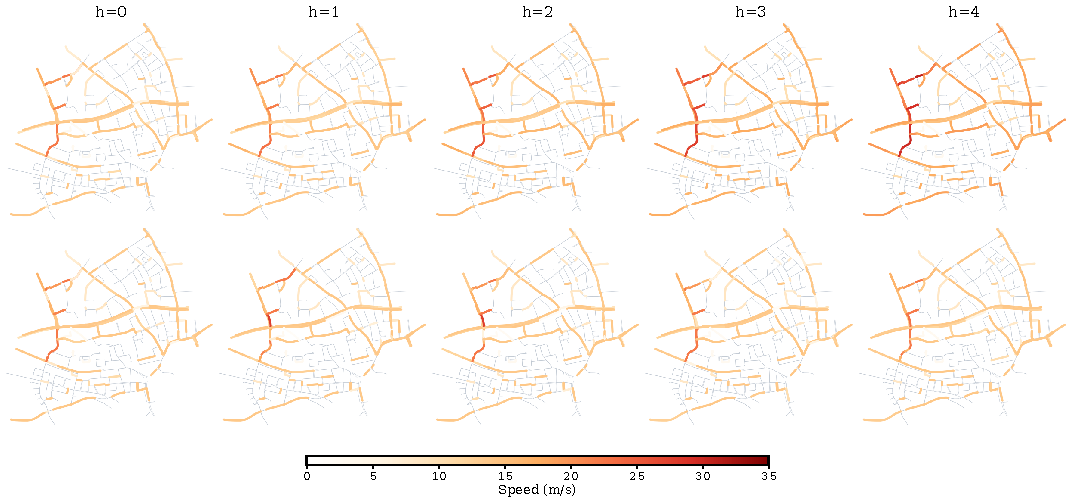
\includegraphics[width=0.75\linewidth]{figure/ingolstadt_construction.pdf}
    \caption{World-model rollout reconstruction on Ingolstadt. Top: speeds decoded from the predicted latent state. Bottom: simulator-observed segment speeds. Columns: prediction horizons \(h=0\) to \(h=4\).}
    \label{fig:ingolstadt-construction}
\end{figure}

\begin{figure}
    \centering
    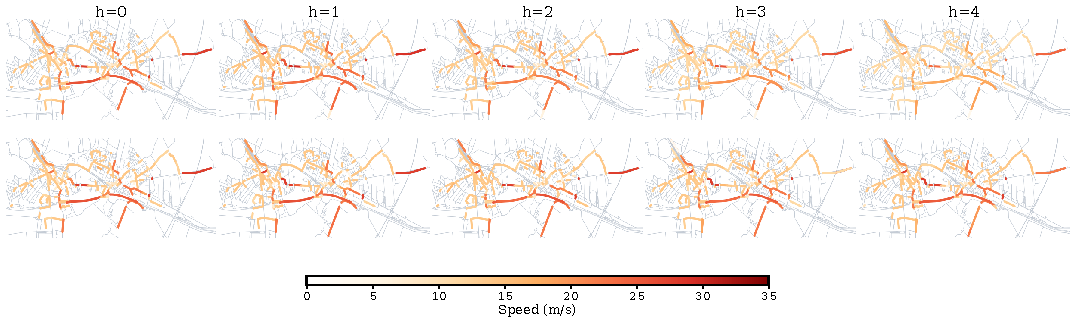
\includegraphics[width=0.75\linewidth]{figure/gretz_construction.pdf}
    \caption{World-model rollout reconstruction on Gretz-Armainvilliers, in the same layout as Figure~\ref{fig:ingolstadt-construction}.}
    \label{fig:gretz-construction}
\end{figure}

\begin{figure}
    \centering
    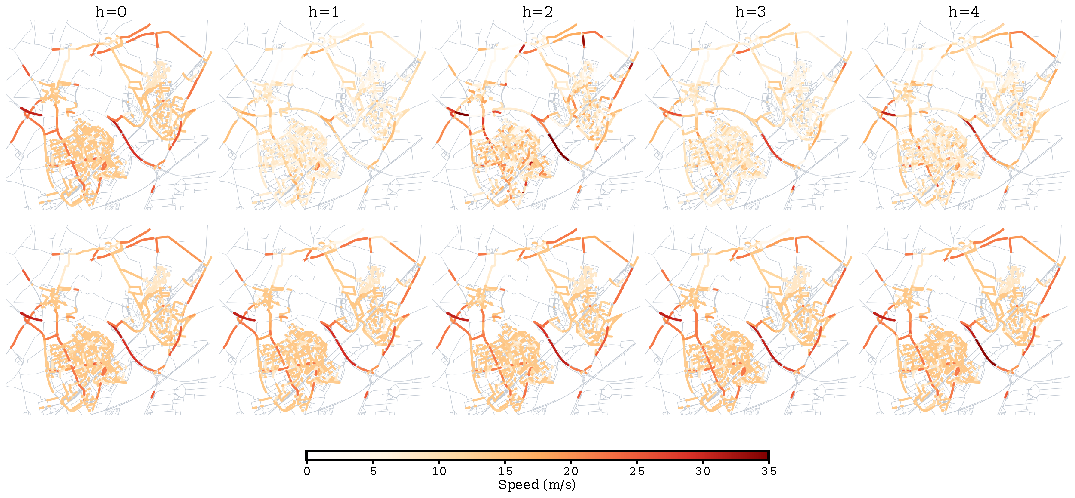
\includegraphics[width=0.75\linewidth]{figure/fontenay_construction.pdf}
    \caption{World-model rollout reconstruction on Fontenay-en-Parisis, in the same layout as Figure~\ref{fig:ingolstadt-construction}.}
    \label{fig:fontenay-construction}
\end{figure}
